\subsubsection{KD-træer}
\label{sec:kdtree}

KD-træer er binære træer, hvilket betyder at hver node maksimalt har to under-noder. K'et i KD-træ er antallet af dimensioner, men i stedet for 3D træ, siger man et 3-dimensionelt KD-træ. KD-træer bruges til at minimere antallet af søgninger, som et givent program skal gennemføre. 

Et KD-træ opbygges ved at have en mængde af værdier, som er usorterede. Disse værdier kan inddeles i et træ, ved at finde et taktisk splittepunkt, som er roden. Herefter går to noder ud fra roden, den venstre har den nedre halvdel af værdierne og den højre har den øvre halvdel. Herefter splittes disse to noder hver for sig igen, og sådan fortsætter træet indtil fastsatte krav nås, hvorefter man så kalder den sidste række af noder for bladene. 

\begin{figure}[H]
  \centering
  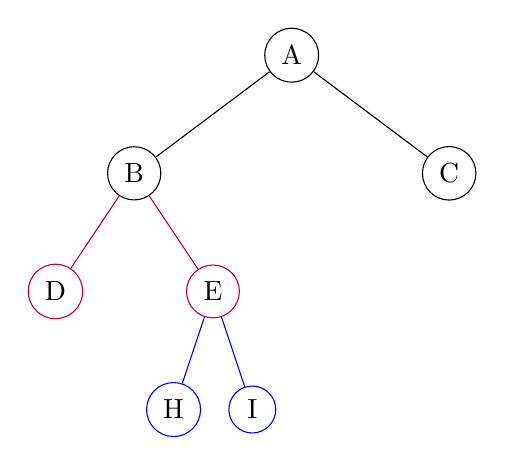
\begin{tikzpicture}[
    level 1/.style={sibling distance=40mm},
    level 2/.style={sibling distance=20mm},
    level 3/.style={sibling distance=10mm},
    every node/.style={draw,circle},
    arrow/.style={edge from parent/.style={draw,-latex}}
  ]
  \node {A}
    child[draw=black] { node{B}
      child[draw=purple] { node{D} }
      child[draw=purple] { node{E}
          child[draw=blue] {node{H}}
          child[draw=blue] {node{I}}
      }
    }
    child[draw=black] { node{C} }
  ;
  \end{tikzpicture}
  \caption{Binært træ}
  \label{fig:binary-tree}
\end{figure}

\begin{figure}[H]
  \begin{subfigure}{0.31\textwidth}
    % \centering
    \begin{tikzpicture}[width=\linewidth, scale=0.9]
      \coordinate (lowlow) at (0,0);
      \coordinate (lowhigh) at (0,5);
      \coordinate (highlow) at (5,0);
      \coordinate (highhigh) at (5,5);

      \coordinate (A1) at (0.4,0);
      \coordinate (A2) at (0,1);
      \coordinate (A3) at (2,0.3);

      \coordinate (B1) at (0.4,5);
      \coordinate (B2) at (2,4);
      \coordinate (B3) at (3,4.3);

      \coordinate (C1) at (5,3.6);
      \coordinate (C2) at (4,3);
      \coordinate (C3) at (4,1.3);

      \coordinate (D1) at (2,3.6);
      \coordinate (D2) at (0.6,3);
      \coordinate (D3) at (1.5,1.3);

      \path[fill=gray!10, draw=black!40] (lowlow) -- (lowhigh) -- (highhigh) -- (highlow) -- (lowlow);
      
      \path[fill=blue!50, draw=blue!20] (A1) -- (A2) -- (A3) -- (A1);
      \path[fill=blue!50, draw=blue!20] (B1) -- (B2) -- (B3) -- (B1);
      \path[fill=blue!50, draw=blue!20] (C1) -- (C2) -- (C3) -- (C1);
      \path[fill=blue!50, draw=blue!20] (D1) -- (D2) -- (D3) -- (D1);
    
      \node [above] at (2.5, 2.25) {$A$};

    \end{tikzpicture}
    \caption{Rod}
    \label{fig:kd-tree-initial}
  \end{subfigure}
  \hspace*{\fill} % separation between the subfigures
  \begin{subfigure}{0.31\textwidth}
    % \centering
    \begin{tikzpicture}[width=\linewidth, scale=0.9]
      \coordinate (lowlow) at (0,0);
      \coordinate (lowhigh) at (0,5);
      \coordinate (highlow) at (5,0);
      \coordinate (highhigh) at (5,5);

      \coordinate (A1) at (0.4,0);
      \coordinate (A2) at (0,1);
      \coordinate (A3) at (2,0.3);

      \coordinate (B1) at (0.4,5);
      \coordinate (B2) at (2,4);
      \coordinate (B3) at (3,4.3);

      \coordinate (C1) at (5,3.6);
      \coordinate (C2) at (4,3);
      \coordinate (C3) at (4,1.3);

      \coordinate (D1) at (2,3.6);
      \coordinate (D2) at (0.6,3);
      \coordinate (D3) at (1.5,1.3);

      \path[fill=gray!10, draw=black!40] (lowlow) -- (lowhigh) -- (highhigh) -- (highlow) -- (lowlow);
      
      \path[fill=blue!50, draw=blue!20] (A1) -- (A2) -- (A3) -- (A1);
      \path[fill=blue!50, draw=blue!20] (B1) -- (B2) -- (B3) -- (B1);
      \path[fill=blue!50, draw=blue!20] (C1) -- (C2) -- (C3) -- (C1);
      \path[fill=blue!50, draw=blue!20] (D1) -- (D2) -- (D3) -- (D1);
      
      \draw [black, thick] (3, 5) -- (3, 0);

      \node [above] at (1.5, 2.25) {$B$};
      \node [above] at (4, 2.25) {$C$};
    \end{tikzpicture}
  \caption{Første itteration}
  \label{fig:kd-tree-itteration}
  \end{subfigure}
  \hspace*{\fill} % separation between the subfigures
  \begin{subfigure}{0.31\textwidth}
    % \centering
    \begin{tikzpicture}[width=\linewidth, scale=0.9]
      \coordinate (lowlow) at (0,0);
      \coordinate (lowhigh) at (0,5);
      \coordinate (highlow) at (5,0);
      \coordinate (highhigh) at (5,5);

      \coordinate (A1) at (0.4,0);
      \coordinate (A2) at (0,1);
      \coordinate (A3) at (2,0.3);

      \coordinate (B1) at (0.4,5);
      \coordinate (B2) at (2,4);
      \coordinate (B3) at (3,4.3);

      \coordinate (C1) at (5,3.6);
      \coordinate (C2) at (4,3);
      \coordinate (C3) at (4,1.3);

      \coordinate (D1) at (2,3.6);
      \coordinate (D2) at (0.6,3);
      \coordinate (D3) at (1.5,1.3);

      \path[fill=gray!10, draw=black!40] (lowlow) -- (lowhigh) -- (highhigh) -- (highlow) -- (lowlow);
      
      \path[fill=blue!50, draw=blue!20] (A1) -- (A2) -- (A3) -- (A1);
      \path[fill=blue!50, draw=blue!20] (B1) -- (B2) -- (B3) -- (B1);
      \path[fill=blue!50, draw=blue!20] (C1) -- (C2) -- (C3) -- (C1);
      \path[fill=blue!50, draw=blue!20] (D1) -- (D2) -- (D3) -- (D1);
      
      \draw [black, thick] (3, 5) -- (3, 0);
      \draw [purple, thick] (0, 3.6) -- (3,  3.6);
      \draw [blue, thick] (0,  1) -- (3,   1);
      
      \node [above] at (4, 2.25) {$C$};
      \node [above] at (1.5, 4.05) {$D$};
      \node [above] at (1.5, 2.05) {$F$};
      \node [above] at (1.5, 0.25) {$G$};
    \end{tikzpicture}
  \caption{Færdigbygget KD-træ}
  \label{fig:kd-tree-finished}
  \end{subfigure}
  \caption{KD-træ}
\end{figure}

En simpel forklaring af et to-dimensionelt KD-træ kan være et program til at finde tallet 100 i en tilfældig mængde fra 1-1000. Roden deles på et bestemt punkt, hvilket i dette tilfælde er midtpå ved 500, og derfor vil den venstre under-node til 'rod-noden' indeholde værdier, der er lig med eller under 500 og det højre barn til indeholde værdier, der er højere end eller lig med 500. Sådan fortsætter programmet med at halvere alle muligheder efter hvert niveau indtil den ønskede værdi er fundet. Denne metode kræver i teorien færre sammenligninger og bør dermed være hurtigerer for store datasæt end hvis man bad et program om at finde et givent tal mellem 1 og 1000, da den, i værste tilfælde, skulle tjekke 999 tal igennem, før den fandt det ønskede nummer.
